\documentclass[11pt,a4paper,oneside]{article}
\usepackage[UTF8,adobefonts]{ctex}

\usepackage{wrapfig}
\usepackage{indentfirst}
\usepackage{amsmath}
\usepackage{float}
\usepackage{ulem}

\usepackage[top=1in,bottom=1in,left=1.25in,right=1.25in]{geometry}

\usepackage{color}
\usepackage{xcolor}

\usepackage{multirow}

\begin{document}

\begin{figure}[H]
 \centering
  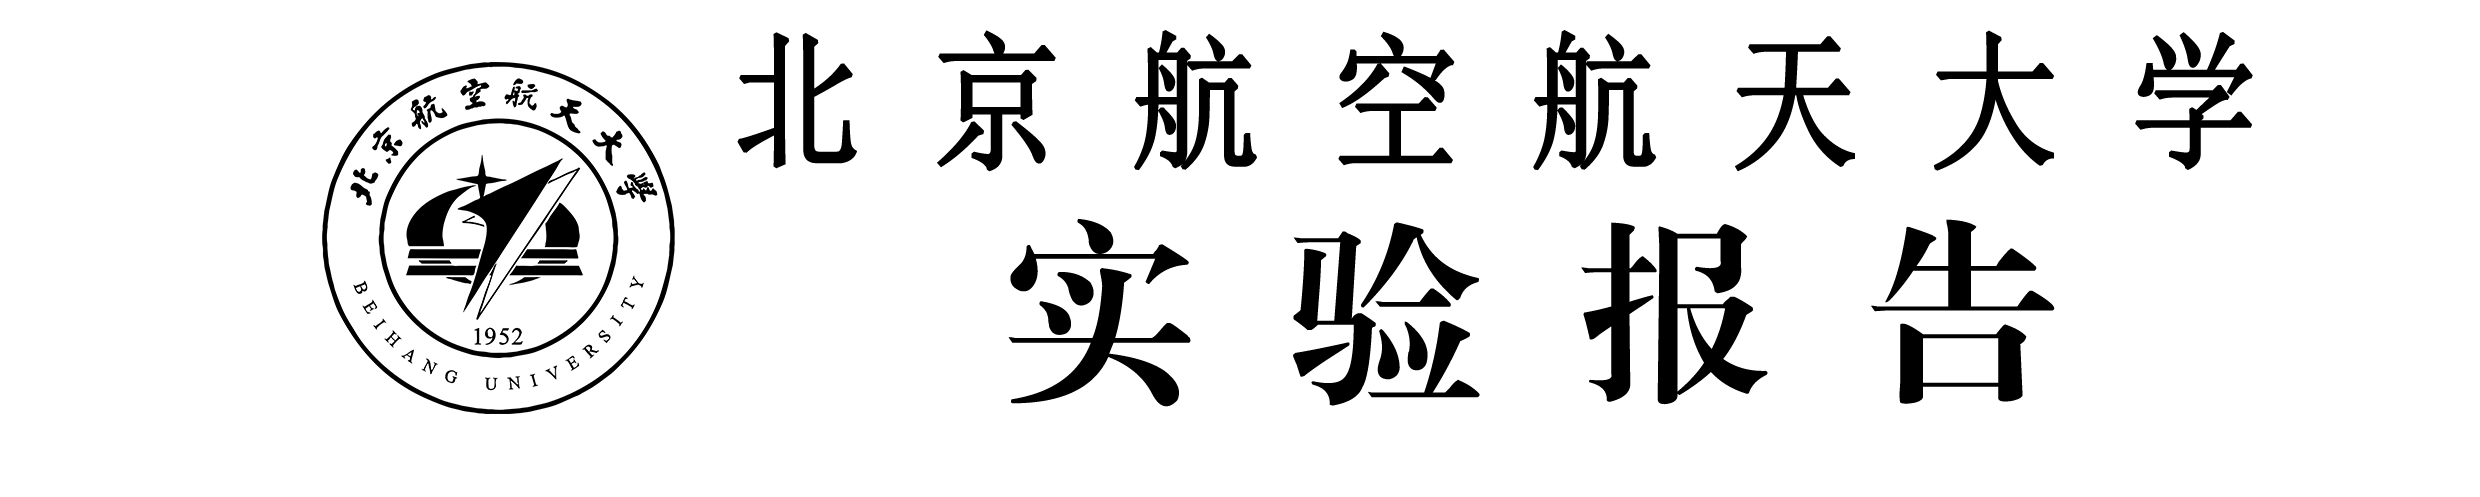
\includegraphics[width=13cm]{表头.png}
\end{figure}
\begin{center}
\textbf{{\large 实验名称:\uline{         伏安法测电阻       }}}
\end{center}

\section*{一、实验目的}
\begin{enumerate}
\item 掌握平衡电桥的原理————零示法与电压比较法;
\item 学习用交换测量法消除系统误差;
\item 学习灵敏度的概念,了解影响电桥灵敏度的因素;
\item 掌握电学实验操作规程,严格规范操作;
\item 学习测量电阻常用的电学仪器仪表的正确使用和箱式电桥的、仪器误差公式;
\item 掌握测量电阻的基本方法,了解不同测量方法各自的适用条件并学习自己设计实验电路;测定高阻、中阻、低阻的阻值及线性、非线性电阻的伏安特性曲线。
\end{enumerate}

\section*{二、实验原理}

所谓伏安法是同时测量电阻两端电压和流过电阻的电流,由欧姆定律
\begin{center}
$ R=\displaystyle\frac{V}{I}$
\end{center}
来求得阻值R。也可用作图法,画出电阻的伏安特性曲线,从曲线上求出电阻的阻值。

\subsubsection*{(1)电路原理}
图4.7.1为伏安法测电阻的两种原理电路,显然由于电表内阻($R_V$、$R_A$)的影响,无论采用电流表内接或电流表外接,都不能严格满足欧姆定律:如采用内接法,则电压表所测电压为$R_L+R_A$ 两端的电压;如采用外接法,则电流表所测电流为流过$R_L$ 与流过$R_V$ 的电流之和。这样就给测量带来了系统误差,称之为“接入误差”或“方法误差”。但此系统误差有规律可循,一旦将误差修正后,即可得到正确结果。
\begin{figure}[htbp]
\centering
  \includegraphics[width=12cm]{伏安法测电阻原理图.png}
\end{figure}

\subsubsection*{(2)伏安法测高电阻与低电阻}
用伏安法测高电阻和低电阻的原理相似,其特殊性表现在前者的工作电流小,而后者的工作电压小。用伏安法测高电阻$(>104\Omega) $时,由于通过电阻的电流太小,一般的电流表测不出来,故采用灵敏电流计;用伏安法测低电阻$(<1\Omega) $时,一般的电压表也难以准确测量,也可采用灵敏电流计测出小电压。为此须先确定灵敏电流计的电流常数$K_i$和内阻$R_g$。测量电路如图4.7.8所示。因检流计不能通过较大的电流,故采用两次分压电路:第一次分压取自滑线变阻器,由电压表读出数据;第二次分压取自$R_1$的端电压。如果条件选择得当,也可以省去第一次分压电路。图4.7.8给出的$E$、$R_1$ 与$R_0$ 的数值只是参考数据,具体数值应根据检流计参数和灵敏度调节旋钮的位置,进行估算和调整,以保证电流适合检流计量程,又便于读数和获得正确的有效数字。

\begin{figure}[htbp]
\centering
  \includegraphics[width=8cm]{半偏法测Rg和Ki.png}
\end{figure}

检流计内阻测量方法为:设定$R_2$ 为0,调节某个元件参数(例如$R_0$),使检流计为满刻度($200div$);再调节$R_2$,并保持$R_1$上的电压不变,使检流计指示值正好为满度之半($10div$),则不难证明:$R_g=R_2$。检流计的电流常数$K_i$即为检流计每小格所代表的电流值,其大小可结合测内阻时,检流计满偏的电压表读数$V$算出。考虑到$R_g$,$R_1$,作用在$R_1$上的电压$V_1$可以充分准确地表示为$V_1=R_1V/(R_0+R_1)$,于是电流常数$K_i$可由下式求出,即
\begin{center}
$K_i=\displaystyle\frac{I_g}{d}=\displaystyle\frac{R_1V}{(R_0+R_1)R_gd}$
\end{center}
式中,$d$是检流计满偏格数。

\subsubsection*{(3)惠斯通电桥测中电阻}
\begin{figure}[htbp]
\centering
  \includegraphics[width=4cm]{惠斯通电桥.png}
\end{figure}
图4.7.9所示为惠斯通提出的电桥电路。它由4个电阻和检流计组成,$R_N$为精密电阻,$R_X$ 为待测电阻。接通电路后,调节$R_1$ 、$R_2$  和$R_N$ ,使检流计中电流为零,电桥达到平衡。易推得电桥平衡条件:
\begin{center}
$R_X=\displaystyle\frac{R_1}{R_2}R_N$
\end{center}
通常称4个电阻为电桥的“臂”,接有检流计的对角线称为“桥”;$R_1/R_2$称为比率或比率臂;$R_N$为标准电阻,称为比较臂;待测电阻$R_X$ 称为测量臂。

由于电桥平衡须由检流计示零表示,故电桥测量方法为零示法,零示法的测量精度较高。又由于电桥测电阻的过程是$D$点电位与$C$点电位进行比较(由示零器指示其比较结果),经过调节直到两点电压为零———电桥达到平衡的过程。

\section*{三、实验仪器}
电阻箱、指针式检流计、固定电阻两个(标称值相同、但不知准确值)、直流稳压电源、滑线变阻器$(200\Omega )$、待测电阻、开关等、QJ45型箱式电桥;QJ19型单双电桥、FMA型电子检流计、滑线变阻器($48\Omega $、$2.5A$)、换向开关、直流稳压电源、电压表两个($0\sim 7.5V$、$0\sim 75V$)、四端钮标准电阻$(0.001\Omega )$、待测低电阻(铜杆)、电流表两个($0\sim 3A$、$0\sim 150mA$)、数显卡尺、待测二极管等。

\section*{四、实验步骤}
\subsubsection*{(1)测线性电阻}
自行选择用伏安法或电桥法测量高电阻、中电阻、低电阻或电表内阻,设计相应的实验电路,确定实验方案,完成电阻的测量。
\subsubsection*{(2)测非线性电阻}
自行设计电路测量二极管的伏安特性。
\begin{enumerate}
\item 测二极管伏安特性曲线时,需根据其正、反向电阻的大小分别采用电流表内接或外接方法。
\item 测量非线性曲线时,需注意不宜均匀取点,而应遵循曲线变化慢处取点疏、曲线变化快处取点密的原则,以便准确绘制曲线。
\item 使用二极管时要注意加在其上的反向电压不得超过最大反向工作电压。
\end{enumerate}
\subsubsection*{(3)数据处理}
\begin{enumerate}
\item 列表记录原始数据;
\item 计算线性电阻的阻值及其不确定度;
\item 用坐标纸绘制二极管伏安特性曲线;
\end{enumerate}

\end{document}